% chktex-file 2% chktex-file 29
% chktex-file 13
\documentclass{report}
\usepackage{setspace}
\usepackage[a4paper, total={7in, 9in}]{geometry}
\usepackage[fleqn]{amsmath}
\usepackage{empheq}
\usepackage{amssymb}
\usepackage{amsthm}
\usepackage{gensymb}
\usepackage[fleqn]{cases}
\usepackage{multicol}
\usepackage{color}
\usepackage{stix}
\usepackage{chngcntr}
\usepackage{tikz}
\usepackage{enumitem}
\usetikzlibrary{calc,matrix,arrows}

\counterwithout{equation}{chapter}
\setlength{\columnseprule}{1pt}
\setlength{\columnsep}{24pt}
\setcounter{chapter}{14}
\hfuzz=100pt

\newtheorem{theorem}{Theorem}

\begin{document}
\newcommand{\sol}[1]{

    \noindent \textbf{Sol.}
}
\newcommand{\prooff}[1]{

    \noindent \textbf{Proof.}
}
\newcommand\m[1]{\begin{pmatrix}#1\end{pmatrix}}
\newcommand\vm[1]{\begin{vmatrix}#1\end{vmatrix}}
\newenvironment{amatrix}[1]{%
    \left(\begin{array}{@{}*{#1}{c}|c@{}}
        }{%
    \end{array}\right)
}
\begin{titlepage}
    \raggedleft{}
    \rule{1pt}{\textheight}
    \hspace{0.02\textwidth}
    \parbox[b]{0.75\textwidth}{

    {\Huge\bfseries Solution Book of \\[0.5\baselineskip] Mathematic}\\[2\baselineskip]
    {\large\textit{Ssnior 2 Part I}}\\[4\baselineskip]
    {\Large\textsc{MELVIN CHIA}}

    \vspace{0.5\textheight}

    {\noindent Written on 9 October 2022}\\[\baselineskip]
    }

\end{titlepage}

\doublespacing{}
\tableofcontents
\singlespacing{}
\newpage

\begin{multicols}{2}
    \subsection*{Solution of the System of Linear Inequalities}

    The system of iniqualities formed by more than one linear inequality is called
    a system of linear inequalities. The solution of a system of linear
    inequalities is the set of all points that satisfy all the inequalities in the
    system, and can be represented by a numberline.

    \subsection{Practice 4}

    Solve the following system of linear inequalities.

    \begin{enumerate}
        \item \begin{numcases}{}
                  3x +2 \geq 2x -2 \\
                  4x -3 > 3x -2
              \end{numcases}
              \sol{}
              \begin{flalign*}
                  (1)          : x & \geq 4 \\
                  (2)          : x & > 1    \\
                  \\
                  \therefore\  x   & > 1
              \end{flalign*}
              \begin{center}
                  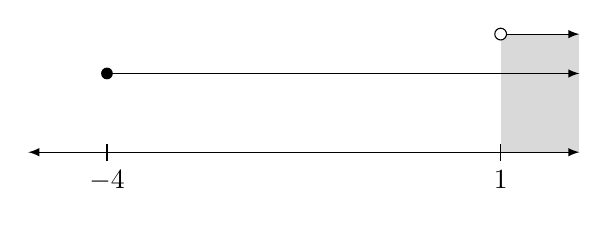
\begin{tikzpicture}
                      \fill[black!15](1,0)rectangle(2,1.5);
                      \draw[latex-latex] (-5,0) -- (2,0) ;
                      \foreach \x in {-4, 1} \draw[shift={(\x,0)},color=black] (0pt,3pt) -- (0pt,-3pt) node[below] {$\x$};
                      \node[circle,fill,inner sep=1.5pt](a)at(-4,1){};
                      \node[circle,draw,fill=white,inner sep=1.5pt](b)at(1,1.5){};
                      \draw[-latex,black](a)--(2,1);
                      \draw[-latex,black](b)--(2,1.5);
                  \end{tikzpicture}
              \end{center}

        \item \begin{numcases}{}
                  5x -4 \leq 2x + 5\\
                  7 -x < 3 + x
              \end{numcases}
              \sol{}
              \begin{flalign*}
                  (1) : 3x       & \leq 9     \\
                  x              & \leq 3     \\
                  (2) : -2x      & < -4       \\
                  x              & > 2        \\
                  \\
                  \therefore\  2 & < x \leq 3
              \end{flalign*}
              \begin{center}
                  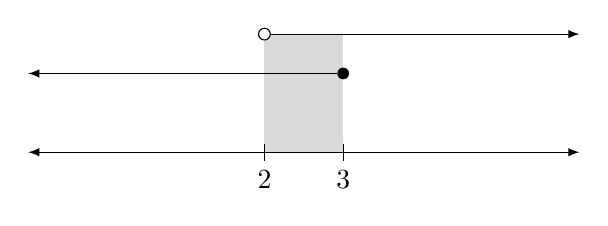
\begin{tikzpicture}
                      \fill[black!15](2,0)rectangle(3,1.5);
                      \draw[latex-latex] (-1,0) -- (6,0) ;
                      \foreach \x in {2, 3} \draw[shift={(\x,0)},color=black] (0pt,3pt) -- (0pt,-3pt) node[below] {$\x$};
                      \node[circle,fill,inner sep=1.5pt](a)at(3,1){};
                      \node[circle,draw,fill=white,inner sep=1.5pt](b)at(2,1.5){};
                      \draw[-latex,black](a)--(-1,1);
                      \draw[-latex,black](b)--(6,1.5);
                  \end{tikzpicture}
              \end{center}

        \item \begin{numcases}{}
                  2 -x < 4 + x\\
                  1 -2x \geq 3x + 11
              \end{numcases}
              \sol{}
              \begin{flalign*}
                  (1) : -2x    & < 2                \\
                  x            & > -1               \\
                  (2) : -5x    & \geq 10            \\
                  x            & \leq -2            \\
                  \\
                  \therefore\  & \text{No solution}
              \end{flalign*}
              \begin{center}
                  \begin{tikzpicture}
                      \draw[latex-latex] (-5,0) -- (2,0) ;
                      \foreach \x in {-2, -1} \draw[shift={(\x,0)},color=black] (0pt,3pt) -- (0pt,-3pt) node[below] {$\x$};
                      \node[circle,fill,inner sep=1.5pt](a)at(-2,1){};
                      \node[circle,draw,fill=white,inner sep=1.5pt](b)at(-1,1){};
                      \draw[-latex,black](a)--(-5,1);
                      \draw[-latex,black](b)--(2,1);
                  \end{tikzpicture}
              \end{center}

        \item $2-x < 2x-7 \leq x-9$
              \sol{}
              \begin{numcases}{}
                  2-x < 2x-7 \\
                  2x-7 \leq x-9
              \end{numcases}
              \begin{flalign*}
                  (1) : -3x    & < -9               \\
                  x            & \geq 3             \\
                  (2) : x      & \leq -2            \\
                  \\
                  \therefore\  & \text{No solution}
              \end{flalign*}
              \begin{center}
                  \begin{tikzpicture}
                      \draw[latex-latex] (-3,0) -- (4,0) ;
                      \foreach \x in {-2, 3} \draw[shift={(\x,0)},color=black] (0pt,3pt) -- (0pt,-3pt) node[below] {$\x$};
                      \node[circle,fill,inner sep=1.5pt](a)at(-2,1){};
                      \node[circle,draw,fill=white,inner sep=1.5pt](b)at(3,1){};
                      \draw[-latex,black](a)--(-3,1);
                      \draw[-latex,black](b)--(4,1);
                  \end{tikzpicture}
              \end{center}
    \end{enumerate}

    \subsection{Exercise 15.2b}

    Solve the following system of linear inequalities.

    \begin{enumerate}

        \item \begin{numcases}{}
                  5 -x < 6\\
                  7 -3x \geq 4
              \end{numcases}
              \sol{}
              \begin{flalign*}
                  (1) : -x        & < 1        \\
                  x               & > -1       \\
                  (2) : -3x       & \geq -3    \\
                  x               & \leq 1     \\
                  \\
                  \therefore\  -1 & < x \leq 1
              \end{flalign*}
              \begin{center}
                  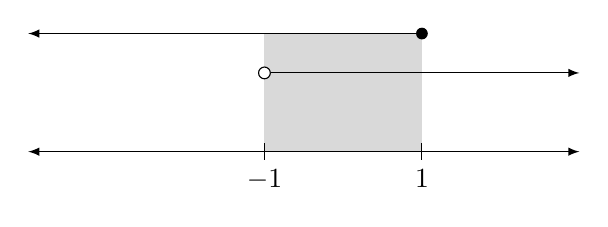
\begin{tikzpicture}
                      \fill[black!15](-1,0)rectangle(1,1.5);
                      \draw[latex-latex] (-4,0) -- (3,0) ;
                      \foreach \x in {-1, 1} \draw[shift={(\x,0)},color=black] (0pt,3pt) -- (0pt,-3pt) node[below] {$\x$};
                      \node[circle,fill,inner sep=1.5pt](a)at(1,1.5){};
                      \node[circle,draw,fill=white,inner sep=1.5pt](b)at(-1,1){};
                      \draw[-latex,black](a)--(-4,1.5);
                      \draw[-latex,black](b)--(3,1);
                  \end{tikzpicture}
              \end{center}

        \item \begin{numcases}{}
                  x + 2 > 0\\
                  2x + 1 \leq 4x -3
              \end{numcases}
              \sol{}
              \begin{flalign*}
                  (1) : x        & > -2    \\
                  (2) : -2x      & \leq -4 \\
                  x              & \geq 2  \\
                  \\
                  \therefore\  x & \geq 2
              \end{flalign*}
              \begin{center}
                  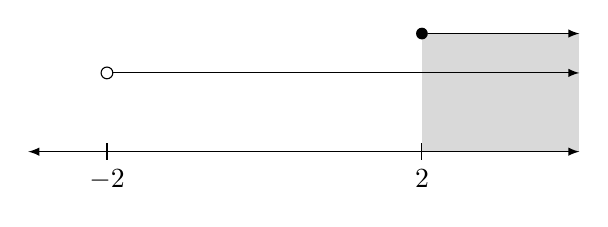
\begin{tikzpicture}
                      \fill[black!15](2,0)rectangle(4,1.5);
                      \draw[latex-latex] (-3,0) -- (4,0) ;
                      \foreach \x in {-2, 2} \draw[shift={(\x,0)},color=black] (0pt,3pt) -- (0pt,-3pt) node[below] {$\x$};
                      \node[circle,fill,inner sep=1.5pt](a)at(2,1.5){};
                      \node[circle,draw,fill=white,inner sep=1.5pt](b)at(-2,1){};
                      \draw[-latex,black](a)--(4,1.5);
                      \draw[-latex,black](b)--(4,1);
                  \end{tikzpicture}
              \end{center}

        \item \begin{numcases}{}
                  3x -1 < 0\\
                  1 -2x \geq 0
              \end{numcases}
              \sol{}
              \begin{flalign*}
                  (1) : 3x       & < 1              \\
                  x              & < \frac{1}{3}    \\
                  (2) : -2x      & \geq -1          \\
                  x              & \leq \frac{1}{2} \\
                  \\
                  \therefore\  x & < \frac{1}{3}
              \end{flalign*}
              \begin{center}
                  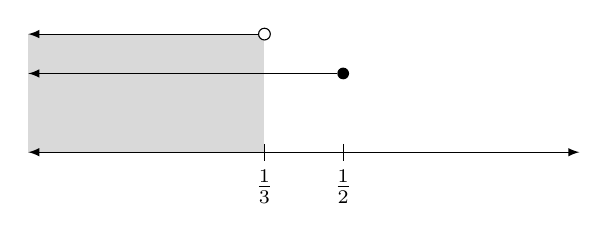
\begin{tikzpicture}
                      \fill[black!15](-6,0)rectangle(-3,1.5);
                      \draw[latex-latex] (-6,0) -- (1,0) ;
                      \foreach \x in {2, 3} \draw[shift={(-\x,0)},color=black] (0pt,3pt) -- (0pt,-3pt) node[below] {$\frac{1}{\x}$};
                      \node[circle,fill,inner sep=1.5pt](a)at(-2,1){};
                      \node[circle,draw,fill=white,inner sep=1.5pt](b)at(-3,1.5){};
                      \draw[-latex,black](a)--(-6,1);
                      \draw[-latex,black](b)--(-6,1.5);
                  \end{tikzpicture}
              \end{center}

        \item \begin{numcases}{}
                  4x -6 \geq 5x\\
                  3x + 5 \leq x + 9
              \end{numcases}
              \sol{}
              \begin{flalign*}
                  (1) : -x       & \geq 6  \\
                  x              & \leq -6 \\
                  (2) : 2x       & \leq 4  \\
                  x              & \geq 2  \\
                  \\
                  \therefore\  x & \leq -6
              \end{flalign*}
              \begin{center}
                  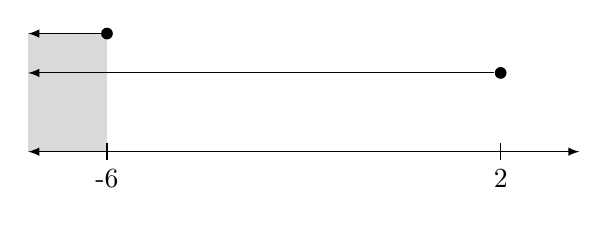
\begin{tikzpicture}
                      \fill[black!15](-7,0)rectangle(-6,1.5);
                      \draw[latex-latex] (-7,0) -- (0,0) ;
                      \draw[shift={(-6,0)},color=black] (0pt,3pt) -- (0pt,-3pt) node[below] {-6};
                      \draw[shift={(-1,0)},color=black] (0pt,3pt) -- (0pt,-3pt) node[below] {2};
                      \node[circle,fill,inner sep=1.5pt](a)at(-6,1.5){};
                      \node[circle,fill,inner sep=1.5pt](b)at(-1,1){};
                      \draw[-latex,black](a)--(-7,1.5);
                      \draw[-latex,black](b)--(-7,1);
                  \end{tikzpicture}
              \end{center}

        \item \begin{numcases}{}
                  2(x+2) > 3x\\
                  6x -8 > 4(x+1)
              \end{numcases}
              \sol{}
              \begin{flalign*}
                  (1): 2x + 4  & > 3x               \\
                  -x           & > -4               \\
                  x            & < 4                \\
                  (2): 6x -  8 & > 4x + 4           \\
                  2x           & > 12               \\
                  x            & > 6                \\
                  \\
                  \therefore\  & \text{No solution}
              \end{flalign*}
              \begin{center}
                  \begin{tikzpicture}
                      \draw[latex-latex] (2,0) -- (9,0);
                      \foreach \x in {4, 6} \draw[shift={(\x,0)},color=black] (0pt,3pt) -- (0pt,-3pt) node[below] {$\x$};
                      \node[circle,fill,inner sep=1.5pt](a)at(4,1){};
                      \node[circle,fill,inner sep=1.5pt](b)at(6,1){};
                      \draw[-latex,black](a)--(2,);
                      \draw[-latex,black](b)--(9,1);
                  \end{tikzpicture}
              \end{center}

    \end{enumerate}
\end{multicols}
\end{document}